\section{Przypadek Testowy 4 - Algorytm genetyczny - zależność PRD od rozmiar populacji}
  \subsection{Cel:}
    Celem tego testu jest sprawdzenie w jakim stopniu rozmiar populacji wpływa na uzyskane PRD. 
    Do testu testu zostaną wykorzystane następujące instancje z \textbf{TSPLIB}
    \begin{enumerate}
        \item berlin52
        \item gr120
        \item ftv70
    \end{enumerate}
    Wszystkie inne argumenty zostały zainicjowane stałymi wartościami optymalnymi dla każdej z instancji. Rozmiary populacji należą do zbioru $ [10,50,100,150,200,250] $
  \subsection{Wyniki: }
    Wyniki testu przedstawione zostały w poniższej tabeli :
    \begin{table}[!ht]
        \centering
        \begin{tabular}{|c | c |}
        \hline
            Rozmiar & PRD \\ \hline
            50 & 19.84\\ \hline
            100 & 14.16\\ \hline
            150 & 6.92\\ \hline
            200 & 6.36 \\ \hline
            250 & 6.57\\ \hline
        \end{tabular}
        \caption{Wyniki otrzymane dla instancji berlin52}
    
      \end{table}
      \begin{table}[!ht]
        \centering
        \begin{tabular}{| c | c |}
        \hline
            Rozmiar & PRD \\ \hline
            50 & 158.72\\ \hline
            100 & 140.95\\ \hline
            150 & 101.75\\ \hline
            200 & 95.82\\ \hline
            250 & 93.08\\ \hline
            
        \end{tabular}
        \caption{Wyniki otrzymane dla instancji gr120}
    
      \end{table}
      \begin{table}[!ht]
        \centering
        \begin{tabular}{|c | c |}
        \hline
            Rozmiar & PRD \\ \hline
            50 & 155.58\\ \hline
            100 & 156.61\\ \hline
            150 & 144.25\\ \hline
            200 & 146.0\\ \hline
            250 & 138.35\\  \hline
        \end{tabular}
        \caption{Wyniki otrzymane dla instancji ftv70}
      \end{table}
  \subsection{Wykresy: }
  \begin{figure}[H]
    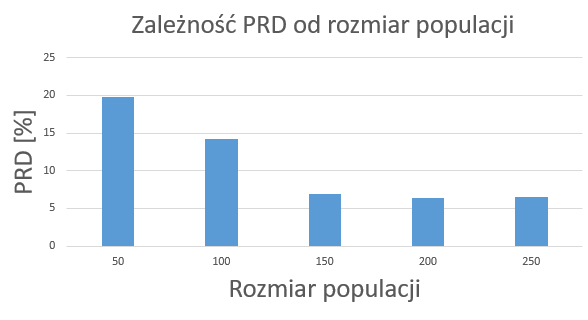
\includegraphics[scale=0.75]{berlin52PRD.png}
    \centering
    \caption{Zależność otrzymanego PRD od rozmiaru populacji dla instancji berlin52}
  \end{figure}
  \begin{figure}[H]
    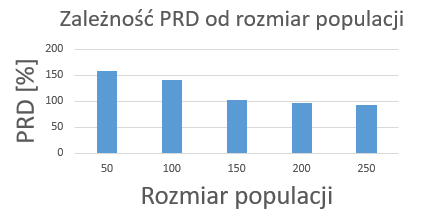
\includegraphics[scale=0.75]{gr120PRD.png}
    \centering
    \caption{Zależność otrzymanego PRD od rozmiaru populacji dla instancji gr120}
  \end{figure}
  \begin{figure}[H]
    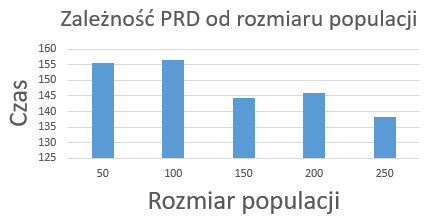
\includegraphics[scale=0.75]{ftv70PRD.png}
    \centering
    \caption{Zależność otrzymanego PRD od rozmiaru populacji dla instancji ftv70}
  \end{figure}
  \subsection{Wnioski: }
      Zauważamy, iż zwiększenie rozmiaru populacji przy stałym utrzymaniu tych samych wariantów wpływa na uzyskanie lepszych wyników, z tą różnicą, że dla instancji asymetrycznych wpływ rozmiaru populacji jest zdecydowanie mniejszy niż dla instancji symetrycznych.
